\documentclass[manuscript,screen,review,anonymous]{acmart}

\settopmatter{printacmref=false, printccs=false}
\renewcommand\footnotetextcopyrightpermission[1]{}

\usepackage{amsmath,amsfonts}
\usepackage{graphicx}
\usepackage{booktabs}
\usepackage{multirow}
\usepackage{array}
\usepackage{makecell}
\usepackage{microtype}
\usepackage{tikz}
\usetikzlibrary{shapes.geometric, arrows.meta, positioning}

\newtheorem{definition}{Definition}
\newtheorem{theorem}{Theorem}
\newtheorem{remark}{Remark}

% Global vertical spacing optimization for page budget
\AtBeginDocument{
  \setlength{\abovedisplayskip}{5pt plus 1pt minus 2pt}
  \setlength{\belowdisplayskip}{5pt plus 1pt minus 2pt}
  \setlength{\abovedisplayshortskip}{0pt plus 1pt}
  \setlength{\belowdisplayshortskip}{3pt plus 1pt minus 1pt}
}

% Standard LaTeX list vertical spacing tightening (safe across ACM classes)
\makeatletter
\def\@listi{\leftmargin\leftmargini
            \parsep 0\p@
            \topsep 2.5\p@ \@plus 1\p@ \@minus 1\p@
            \itemsep 1.5\p@ \@plus 0.5\p@}
\let\@listI\@listi
\setlength{\abovecaptionskip}{4pt plus 1pt minus 1pt}
\setlength{\belowcaptionskip}{4pt plus 1pt minus 1pt}
\makeatother

\begin{document}

\title[Beyond the Illusion of Recourse]{Beyond the Illusion of Recourse: An Auditable Dual-Pathway Architecture for Actionable Credit Governance}

\author{Anonymous Author(s)}
\affiliation{%
  \institution{Affiliation Omitted for Double-Blind Review}
  \country{}
}

\begin{abstract}
Post-hoc counterfactual explainability promises actionable algorithmic recourse for adverse automated decisions. In practical credit underwriting, however, standard counterfactuals frequently produce inexecutable recommendations: modifying immutable bureau records, erasing past delinquencies, or prescribing impossible cash flows.

To address this, we introduce FairRecourse, an auditable dual-pathway recourse architecture for regulated consumer lending. Rather than treating recourse as a borrower-only optimization problem, we challenge the unilateral assumption in credit underwriting: when an applicant's profile cannot be resolved through feasible borrower actions alone ($\mathcal{F}_B(x) = \emptyset$), an institution-aware framework transitions to an admissible institutional counter-offer ($\mathcal{F}_I(x) \neq \emptyset$). We formalize the Policy and Constraint Layer (PCL) to enforce domain invariants, directional monotonicity, and execution horizons. When historical credit bureau records induce an Immutability Deadlock, our framework computes an expected-loss-constrained exposure scaling factor ($\alpha^* = \tau / PD$) based on the applicant's calibrated probability of default ($PD$) to restructure the facility limit to preserve the institution's target risk bound.

We evaluate our framework against Diverse Counterfactual Explanations (DiCE) across three sovereign credit benchmarks: Statlog German Credit ($N=1,000$, EUR), FICO HELOC ($N=10,000$, USD), and an Indian credit bureau benchmark (CIBIL Retail, $N=51,336$, INR). Across 670 audited borderline applicants ($PD \in [0.405, 0.500]$), unconstrained DiCE produced 967 policy violations across 87.9\% of cases, while borrower-side recourse alone collapsed to 3.8\% on HELOC and 0.0\% on CIBIL. FairRecourse yields zero policy violations and achieves 100.0\% total admissible pathway coverage ($S_R$). When borrower action is feasible, it provides actionable recourse ($S_B = 100.0\%$ in German Credit, $3.8\%$ in HELOC); when borrowers are deadlocked, it provides institutional counter-offers ($S_I = 96.2\%$ in HELOC, $100.0\%$ in CIBIL) with modest credit haircuts between 1.3\% and 20.0\%. Sensitivity analysis across horizons ($H_{\max} \in \{6, 12, 18, 24, 36\}$ months) demonstrates how temporal constraints shift the burden between individual action and institutional adjustment.
\end{abstract}

\begin{CCSXML}
<ccs2012>
   <concept>
       <concept_id>10010147.10010257</concept_id>
       <concept_desc>Computing methodologies~Machine learning</concept_desc>
       <concept_significance>500</concept_significance>
       </concept>
   <concept>
       <concept_id>10003456.10003457.10003527</concept_id>
       <concept_desc>Social and professional topics~Socio-technical systems</concept_desc>
       <concept_significance>500</concept_significance>
       </concept>
   <concept>
       <concept_id>10010405.10003550.10003551</concept_id>
       <concept_desc>Applied computing~Operations research</concept_desc>
       <concept_significance>300</concept_significance>
       </concept>
 </ccs2012>
\end{CCSXML}

\ccsdesc[500]{Computing methodologies~Machine learning}
\ccsdesc[500]{Social and professional topics~Socio-technical systems}
\ccsdesc[300]{Applied computing~Operations research}

\keywords{Algorithmic Recourse, Explainable AI, Credit Risk Governance, Counterfactual Explanations, Algorithmic Auditing, Model Risk Management, Sociotechnical Systems}

\maketitle

\section{Introduction}

\subsection{The Operationalization Gap in Algorithmic Recourse}
Over the past decade, explainable artificial intelligence (XAI) literature has shifted its primary paradigm from passive feature attributions---such as SHAP~\cite{lundberg2017unified} or LIME~\cite{ribeiro2016why}---toward actionable algorithmic recourse~\cite{wachter2017counterfactual,ustun2019actionable,karimi2021algorithmic}. The guiding premise of algorithmic recourse is normative: any decision system that denies an individual a consequential economic benefit, such as a mortgage or consumer credit facility, must provide an actionable path of intervention through which the applicant can overturn that adverse determination.

However, a fundamental disconnect persists between the theoretical formulation of counterfactual explanations in computer science and the regulatory, operational, and financial realities of retail banking. Counterfactual generation is conventionally formulated as an optimization problem over a continuous manifold:
\begin{equation}
\min_{x^* \in \mathcal{X}} \operatorname{dist}(x, x^*) \quad \text{subject to} \quad f(x^*) \le \tau
\label{eq:standard_recourse}
\end{equation}
where $\operatorname{dist}(\cdot)$ represents a distance metric, $f: \mathcal{X} \to [0, 1]$ outputs the calibrated probability of default $PD(x)$, and $\tau$ denotes the operational approval threshold.

In retail lending, underwriting models evaluate complex, high-dimensional profiles containing past credit histories, legal constraints, and non-linear financial ratios, typically using gradient-boosted decision trees (GBDTs)~\cite{ke2017lightgbm}. When general-purpose counterfactual optimizers---such as Diverse Counterfactual Explanations (DiCE)~\cite{mothilal2020dice} or CARLA implementations~\cite{pawelczyk2021carla}---are deployed on credit data without domain constraints, they exploit mathematical shortcuts along the loss surface. These shortcuts routinely manifest as inexecutable instructions:
\begin{enumerate}
    \item Mutating protected demographic classifications;
    \item Arbitrarily erasing historical bureau delinquency events (e.g., advising an applicant to eliminate past 60-day delinquencies);
    \item Fabricating fractional values on discrete counts (e.g., recommending $2.37$ open credit lines);
    \item Prescribing debt paydowns requiring financial commitments exceeding disposable income over realistic planning windows.
\end{enumerate}

\subsection{The Optimization Deadlock}
Beyond generating physically inadmissible recommendations, existing recourse frameworks suffer from an unaddressed structural failure: \textbf{The Optimization Deadlock}. In real-world underwriting, a significant fraction of adverse loan applicants possess established, deeply anchored credit impairments (e.g., recent bankruptcies, low external bureau scores, or high debt-to-income ratios). For these applicants, the decision boundary cannot be traversed through actionable adjustments to mutable features within viable thresholds.

Current counterfactual frameworks treat optimization deadlocks as terminal failures, returning an empty set that forces an outright denial ($\text{Recourse}(x) = \emptyset$). While human loan officers routinely adjust credit limits or loan terms to approve borderline applicants, algorithmic recourse research has focused almost entirely on requiring applicants to change their own attributes. We bridge this gap by formalizing a dual-pathway framework that combines borrower-side actions with institution-side credit limit adjustments.

\subsection{Formal Contributions}
To connect post-hoc algorithmic explainability with responsible credit risk management and applicable banking requirements across global jurisdictions, we propose FairRecourse and advance four formal contributions:
\begin{enumerate}
    \item \textbf{The Policy and Constraint Layer (PCL):} We formalize a deterministic verification engine that functions as an auditable firewall against unconstrained counterfactual search. The PCL explicitly encodes domain immutability allowlists, directional monotonicity boundaries (prohibiting debt accumulation or asset depletion), discrete integrality of trade counts, and physical bounds as a coupled mathematical predicate $\mathcal{C}(x, x')$.
    \item \textbf{Risk-Constrained Exposure Sizing ($\alpha^*$):} We challenge the borrower-only assumption in credit recourse. Anchored in the fundamental expected loss invariant ($EL = PD \times LGD \times EAD$), we prove that when borrower-side adjustments encounter an immutability deadlock ($\mathcal{F}_B(x) = \emptyset$), scaling credit exposure via $\alpha^* = \min(1.0, \tau / PD(x))$ preserves the lender's target risk bound, establishing a closed-form bridge to an institutional counter-offer ($\mathcal{F}_I(x) \neq \emptyset$).
    \item \textbf{Temporal Solvency \& Feasibility Metrics:} We derive a dynamic translation function converting abstract utilization changes into nominal currency commitments bounded by realistic credit ceilings ($\widehat{\text{Limit}}(x) \le 6 \times \text{Income}$). We formalize the Execution Horizon metric bounded by a baseline planning parameter $H \le H_{\max}$ ($H_{\max} = 24$ months, with sensitivity evaluated up to 36 months) and evaluate recourse stability under stochastic execution perturbations as an explicit probability metric $\mathcal{R}_{\text{stab}}$.
    \item \textbf{Multi-Regime Empirical Audit ($N=670$):} We evaluate the framework across three representative credit regimes: Statlog German Credit ($N=34$ marginal applicants), FICO HELOC ($N=260$), and Indian CIBIL Retail ($N=376$). We demonstrate that while baseline counterfactuals produce up to 93.8\% policy-invalid outcomes, FairRecourse achieves 100.0\% total admissible coverage ($S_R = S_B + S_I$) by formally shifting deadlocked applicants into an auditable institutional pathway.
\end{enumerate}

\subsection{Research Questions}
To evaluate FairRecourse, we formulate three operational research questions:
\begin{itemize}
    \item[\textbf{RQ1:}] \emph{How frequently do unconstrained counterfactuals violate predefined credit-domain constraints across diverse retail credit regimes?}
    \item[\textbf{RQ2:}] \emph{How do domain and execution constraints affect the availability of feasible borrower-side recourse across different credit-data regimes?}
    \item[\textbf{RQ3:}] \emph{When borrower-side recourse is infeasible, can institution-side exposure scaling provide an admissible alternative under a specified expected-loss constraint?}
\end{itemize}

\subsection{Sociotechnical Framing: Allocating the Burden of Recourse}
Standard algorithmic recourse implicitly adopts a unilateral, borrower-centric stance: the model and the requested facility terms are treated as fixed, while the applicant is expected to alter their life circumstances to accommodate the algorithm. This framing produces three sociotechnical distortions:
\begin{enumerate}
    \item \textbf{Model Space vs. Action Space Divergence:} A counterfactual can be valid in model space ($f(x') \le \tau$) while being invalid in action space ($\mathcal{C}(x, x') = 0$). Conflating mathematical loss minimization with human executability produces an illusion of recourse.
    \item \textbf{Borrower Feasibility vs. Institutional Admissibility:} An action can be theoretically feasible for the borrower but inadmissible to the institution, or conversely, an applicant may be structurally unable to act unilaterally while the institution retains flexible contractual levers to accommodate them safely.
    \item \textbf{Obscuring Institutional Responsibility:} When borrower-side recourse is infeasible ($\mathcal{F}_B(x) = \emptyset$), treating the outcome as a terminal denial obscures the institution's role in determining the decision space. Retail credit is a bilateral contract; the lender defines the requested facility size, tenure, and risk margin. 
\end{enumerate}

\section{Background and Related Work}

\subsection{Foundations of Algorithmic Recourse}
To ground FairRecourse within the broader explainability literature, we review the technical evolution of recourse from unconstrained distance minimization toward domain-aware optimization. Algorithmic recourse formalizes post-hoc explainability by identifying minimal, actionable feature interventions that overturn an adverse classification. Wachter et al.~\cite{wachter2017counterfactual} formulated counterfactual search as continuous distance minimization balanced against prediction loss. Ustun et al.~\cite{ustun2019actionable} introduced actionable recourse using integer programming over linear models to restrict perturbations to user-actionable subsets.

To address non-linear model architectures, Mothilal et al.~\cite{mothilal2020dice} developed DiCE, using gradient or genetic optimization over prediction loss, proximity, and diversity---later benchmarked across tree ensembles and generative priors via CARLA~\cite{pawelczyk2021carla}. Joshi et al.~\cite{joshi2019towards} and Rawal and Lakkaraju~\cite{rawal2020individually} examined actionable recourse preservation, while Upadhyay et al.~\cite{upadhyay2021robust} addressed recourse robustness under model shifts.

\subsection{Actionability, Causal Dependencies, and Fairness}
Causal recourse frameworks~\cite{karimi2021causal,mahajan2019preserving} established that feature modifications must respect structural causal relationships to avoid physically incoherent interventions. Subsequent works investigated fairness disparities in recourse availability, demonstrating that disadvantaged demographic groups often face systematically higher recourse costs~\cite{vonkugelgen2022fairness,gupta2019equalizing,sharma2020certkai,barocas2020hidden,venkatasubramanian2020philosophical}.

These works progressively incorporate actionability, causal dependencies, and fairness. However, they primarily model recourse as intervention over applicant attributes. They do not jointly model borrower-side feasibility, execution-horizon constraints, and institution-controlled exposure adjustments within a single recourse framework.

\subsection{Credit Governance and Institutional Decision-Making}
We use laws and regulatory instruments as context for selecting the constraints evaluated in this study. The rules implemented in FairRecourse are a limited computational specification, not an exhaustive legal interpretation or proof of compliance with every requirement.

In the United States, credit decision governance is informed by the Equal Credit Opportunity Act (ECOA, 15 U.S.C. \S~1691), implemented via Regulation B (12 C.F.R. Part 1002), and the Fair Credit Reporting Act (FCRA, 15 U.S.C. \S~1681). Under Regulation B, conditioning credit determinations on protected demographic characteristics is prohibited, motivating our demographic immutability predicate. Furthermore, 12 C.F.R. \S~1002.9(a)(1)(iv) recognizes conditional counter-offers as an established credit practice, while Consumer Financial Protection Bureau (CFPB) Circular 2022-03~\cite{cfpb2022circular} underscores that creditors cannot evade adverse action explanation requirements through algorithmic complexity.

In the European Union, the General Data Protection Regulation (GDPR Article 22)~\cite{gdpr2016} and the European Union Artificial Intelligence Act (EU AI Act, Regulation 2024/1689, Annex III.5b)~\cite{euaiact2024} classify automated credit scoring as high-risk, emphasizing transparency, contestability, and human oversight. In India, the Reserve Bank of India (RBI) Digital Lending Directions (2022)~\cite{rbi2022digitallending} similarly emphasize auditable governance in automated credit assessment.

Under Basel III/IV Internal Ratings-Based (IRB) standards~\cite{bcbs2017basel}, institutions evaluate retail credit risk through Expected Loss: $EL = PD \times LGD \times EAD$, where $PD \in [0, 1]$ is the calibrated default probability, $LGD \in [0, 1]$ is Loss Given Default, and $EAD \in \mathbb{R}^+$ is nominal Exposure at Default. When an applicant's default risk exceeds the institution's internal risk threshold $\tau$, extending the requested facility $EAD_0$ breaches risk appetite. By scaling $EAD$, institutions preserve target expected loss without requiring unilateral borrower modification.

\subsection{Identifying the Operational Gap}
While credit-limit adjustments and loan restructuring are established lending practices in conventional manual underwriting, existing algorithmic recourse frameworks place the entire burden of intervention on changing the applicant's own attributes. Our contribution lies in formally integrating institution-controlled exposure adjustment into an automated algorithmic recourse optimization pipeline—coupling it with a deterministic borrower-feasibility test, an institutional expected-loss constraint check, and an auditable policy trail. Table~\ref{tab:literature_matrix} summarizes how FairRecourse compares with prior literature across operational desiderata.

\begin{table}[!htbp]
\centering
\caption{Systematic Literature Matrix: Comparing Recourse Frameworks Across Operational Desiderata.}
\label{tab:literature_matrix}
\small
\setlength{\tabcolsep}{4pt}
\resizebox{\columnwidth}{!}{%
\begin{tabular}{lcccccc}
\toprule
\textbf{Literature / Framework} & \textbf{Optimization} & \textbf{Actionability} & \textbf{Causal / Relat.} & \textbf{Temporal} & \textbf{Institutional} & \textbf{Credit Domain} \\
 & \textbf{Algorithm} & \textbf{Constraints} & \textbf{Constraints} & \textbf{Solvency ($H$)} & \textbf{Pathway ($S_I$)} & \textbf{Invariants} \\
\midrule
Wachter et al. (2017)~\cite{wachter2017counterfactual} & Distance-based & Partial & -- & -- & -- & -- \\
Ustun et al. (2019)~\cite{ustun2019actionable} & Integer Prog. & \checkmark & -- & -- & -- & Partial \\
DiCE (Mothilal et al., 2020)~\cite{mothilal2020dice} & Genetic/Grad. & \checkmark & -- & -- & -- & -- \\
Causal Recourse (Karimi et al., 2021)~\cite{karimi2021causal} & Structural & \checkmark & \checkmark & -- & -- & -- \\
Fairness/Recourse (von K\"ugelgen et al., 2022)~\cite{vonkugelgen2022fairness} & Causal/Fair & \checkmark & \checkmark & -- & -- & Partial \\
\midrule
\textbf{FairRecourse (This Work)} & \textbf{Dual-Pathway} & \textbf{\checkmark} & \textbf{\checkmark} & \textbf{\checkmark} & \textbf{\checkmark} & \textbf{\checkmark} \\
\bottomrule
\end{tabular}%
}
\end{table}

\section{Problem Formulation}

\subsection{Credit Decision Setting}
Let $x \in \mathcal{X}$ denote an applicant's feature vector in a $d$-dimensional space. The underwriting engine evaluates $x$ via $f(x) = PD(x) \in [0, 1]$. An adverse determination occurs when $PD(x) > \tau$. All monetary quantities are expressed in native currency (EUR for German Credit, USD for HELOC, and INR for CIBIL).

\subsection{Borrower Feasible Set}
\begin{definition}[Borrower Feasible Set]
Let $\mathcal{C}(x, x') \in \{0, 1\}$ denote a composite domain constraint predicate. The \textbf{Borrower Feasible Set} $\mathcal{F}_B(x)$ is:
\begin{equation}
\mathcal{F}_B(x) = \left\{ x' \in \mathcal{X} \;\middle|\; f(x') \le \tau, \; \mathcal{C}(x, x') = 1 \right\}
\label{eq:borrower_feasible_set}
\end{equation}
\end{definition}

\begin{definition}[Immutability Deadlock]
An applicant $x$ experiences an \textbf{Immutability Deadlock} when no actionable modification can satisfy the approval threshold under the domain constraint predicate: $\mathcal{F}_B(x) = \emptyset$.
\end{definition}

\subsection{Institutional Feasible Set}
\begin{definition}[Institutional Feasible Set]
Let $EAD_0$ denote the requested credit facility limit. When borrower-side recourse is deadlocked ($\mathcal{F}_B(x) = \emptyset$), the institution evaluates facility restructuring $EAD' = \alpha EAD_0$ subject to preserving portfolio Expected Loss within institutional risk tolerance:
\begin{equation}
EL' = PD(x) \times LGD \times (\alpha EAD_0) \le EL_{\max} = \tau \times LGD \times EAD_0
\label{eq:institutional_el}
\end{equation}
The set of admissible institutional counter-offers $\mathcal{F}_I(x)$ is defined over $\alpha \in [\alpha_{\min}, 1.0]$:
\begin{equation}
\mathcal{F}_I(x) = \left\{ \alpha^* \in [\alpha_{\min}, 1.0] \;\middle|\; \alpha^* = \min\left(1.0, \, \frac{\tau}{PD(x)}\right) \right\}
\label{eq:institutional_pathway}
\end{equation}
where $\alpha_{\min} = 0.80$ defines an operational haircut viability floor capping the maximum automated facility reduction at 20\%.
\end{definition}

\subsection{Dual-Pathway Recourse}
\begin{definition}[Dual-Pathway Recourse Function]
The complete \textbf{Dual-Pathway Recourse Function} $R(x)$ bridges borrower agency with institutional exposure adjustment:
\begin{equation}
R(x) = \begin{cases}
R_B(x), & \mathcal{F}_B(x) \neq \emptyset \\
R_I(x), & \mathcal{F}_B(x) = \emptyset \text{ and } \mathcal{F}_I(x) \neq \emptyset \\
\text{Human Escalation}, & \mathcal{F}_B(x) = \emptyset \text{ and } \mathcal{F}_I(x) = \emptyset
\end{cases}
\label{eq:dual_pathway}
\end{equation}
where $R_B(x) = \arg\min_{x' \in \mathcal{F}_B(x)} \operatorname{Cost}(x, x')$ produces an actionable Borrower Action Plan, and $R_I(x)$ issues a risk-constrained exposure-scaling counter-offer certificate.
\end{definition}

\section{FairRecourse Architecture}

Figure~\ref{fig:architecture} illustrates the system pipeline.

\begin{figure}[t]
\centering
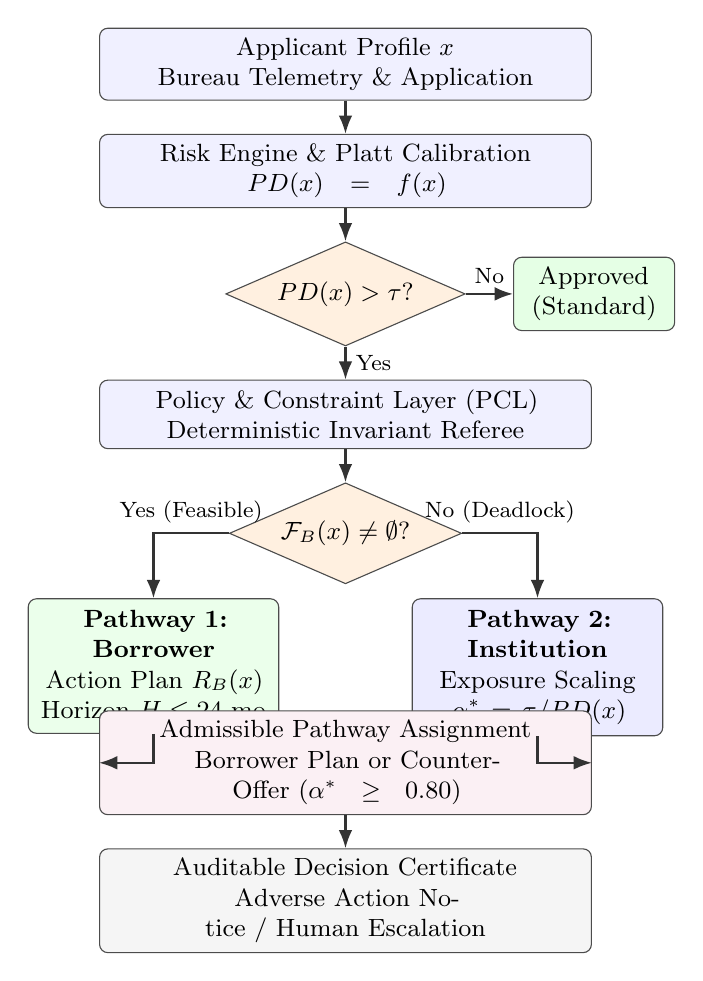
\begin{tikzpicture}[
    node distance=0.42cm,
    box/.style={rectangle, draw=black!70, rounded corners=3pt, align=center, fill=blue!6, inner sep=3.5pt, font=\small, text width=6.0cm},
    decision/.style={diamond, draw=black!70, aspect=2.3, align=center, fill=orange!12, inner sep=2.5pt, font=\small},
    branch/.style={rectangle, draw=black!70, rounded corners=3pt, align=center, inner sep=4pt, font=\small, text width=2.9cm},
    arrow/.style={-Latex, thick, draw=black!80}
]
% Flowchart Nodes
\node[box] (input) {Applicant Profile $x$\\Bureau Telemetry \& Application};
\node[box, below=of input] (model) {Risk Engine \& Platt Calibration\\$PD(x) = f(x)$};
\node[decision, below=of model] (check) {$PD(x) > \tau$?};
\node[box, right=0.6cm of check, text width=1.8cm, fill=green!10] (approved) {Approved\\(Standard)};
\node[box, below=of check] (pcl) {Policy \& Constraint Layer (PCL)\\Deterministic Invariant Referee};
\node[decision, below=of pcl] (feas) {$\mathcal{F}_B(x) \neq \emptyset$?};
\node[branch, below left=0.5cm and 0.1cm of feas, fill=green!8] (borrower) {\textbf{Pathway 1: Borrower}\\Action Plan $R_B(x)$\\Horizon $H \le 24$ mo};
\node[branch, below right=0.5cm and 0.1cm of feas, fill=blue!8] (inst) {\textbf{Pathway 2: Institution}\\Exposure Scaling\\$\alpha^* = \tau / PD(x)$};
\node[box, below=1.6cm of feas, fill=purple!6] (outcome) {Admissible Pathway Assignment\\Borrower Plan or Counter-Offer ($\alpha^* \ge 0.80$)};
\node[box, below=of outcome, fill=gray!8] (audit) {Auditable Decision Certificate\\Adverse Action Notice / Human Escalation};

% Connectors
\draw[arrow] (input) -- (model);
\draw[arrow] (model) -- (check);
\draw[arrow] (check) -- node[above, font=\footnotesize] {No} (approved);
\draw[arrow] (check) -- node[right, font=\footnotesize] {Yes} (pcl);
\draw[arrow] (pcl) -- (feas);
\draw[arrow] (feas) -| node[above, pos=0.25, font=\footnotesize] {Yes (Feasible)} (borrower);
\draw[arrow] (feas) -| node[above, pos=0.25, font=\footnotesize] {No (Deadlock)} (inst);
\draw[arrow] (borrower) |- (outcome);
\draw[arrow] (inst) |- (outcome);
\draw[arrow] (outcome) -- (audit);
\end{tikzpicture}
\caption{The FairRecourse Dual-Pathway Architecture. When domain constraints induce an Immutability Deadlock ($\mathcal{F}_B(x) = \emptyset$), the framework activates Pathway 2, sizing institutional exposure ($\alpha^*$) to preserve the target expected-loss bound.}
\label{fig:architecture}
\end{figure}

\subsection{Policy and Constraint Layer (PCL)}
The coupled constraint set is the conjunction of all conditions that a candidate borrower intervention must satisfy simultaneously. A candidate is admissible only if it preserves immutable attributes, respects directional relationships, obeys discrete and range constraints, and remains executable within the specified financial horizon:
\begin{equation}
\mathcal{C}(x, x') \iff \Phi_{\text{immut}}(x, x') \land \Phi_{\text{monot}}(x, x') \land \Phi_{\text{discr}}(x') \land \Phi_{\text{bounds}}(x') \land \Phi_{\text{solv}}(x, x')
\end{equation}

\subsubsection{Immutability Predicate ($\Phi_{\text{immut}}$)}
Let $\mathcal{I} \subseteq \{1, \dots, d\}$ denote the index set of immutable features, encompassing protected demographic attributes (e.g., age, gender) and historical credit bureau telemetry (e.g., inquiry recency, delinquency records, trade tenure). For any candidate intervention $x'$, immutable attributes must remain unchanged: $\Phi_{\text{immut}}(x, x') \iff x'_j = x_j, \; \forall j \in \mathcal{I}$. In our numerical implementation, this is evaluated as $|x'_j - x_j| \le 10^{-4}$ to accommodate floating-point representations. Any candidate perturbing an index in $\mathcal{I}$ violates the defined immutability constraint.

\subsubsection{Directional Monotonicity Predicate ($\Phi_{\text{monot}}$)}
Let $\mathcal{M}_{\text{adverse}}$ denote the index set of financial liabilities, revolving debt balances, and utilization burdens. Let $\mathcal{M}_{\text{asset}}$ denote positive assets (e.g., liquid savings). We enforce:
\begin{equation}
\Phi_{\text{monot}}(x, x') \iff \left( \forall j \in \mathcal{M}_{\text{adverse}}, \; x'_j \le x_j \right) \land \left( \forall k \in \mathcal{M}_{\text{asset}}, \; x'_k \ge x_k \right)
\end{equation}

\subsubsection{Integrality and Range Bounds ($\Phi_{\text{discr}}, \Phi_{\text{bounds}}$)}
Discrete trade and inquiry counts must satisfy integer constraints ($|x'_j - \operatorname{round}(x'_j)| \le 10^{-3}$), while percentage attributes remain bounded in $[0, 100]$.

\subsection{Temporal Solvency and Execution Horizon}
In retail credit files, an individual's explicit credit card limit is often unobserved in bureau aggregates. FairRecourse dynamically estimates the individual's credit limit $\widehat{\text{Limit}}(x)$ by inverting observed revolving utilization $U(x)$:
\begin{equation}
\widehat{\text{Limit}}(x) = \begin{cases}
\min\left(\max\left(\frac{D_{\text{revolving}}(x)}{U(x) / 100}, \, C_{\min}\right), \, 6 \times \text{Income}_{\text{monthly}}(x)\right), & \text{if } U(x) \ge 1.0 \land D_{\text{revolving}} > 0 \\
3 \times \text{Income}_{\text{monthly}}(x), & \text{otherwise}
\end{cases}
\end{equation}
where $C_{\min}$ is the regional minimum credit floor (EUR 500, USD 500, INR 5,000). The ceiling $6 \times \text{Income}_{\text{monthly}}$ imposes an institutional safeguard against inflating limits on near-zero balances.

The total nominal capital shift $\Delta \Omega(x, x')$ required to execute $x'$ aggregates savings accumulation, debt paydowns, and credit line reductions:
\begin{equation}
\Delta \Omega(x, x') = \max(0, x'_{\text{savings}} - x_{\text{savings}}) + \max(0, x_{\text{debt}} - x'_{\text{debt}}) + \sum_{j \in \mathcal{U}} \left( \frac{\max(0, x_j - x'_j)}{100} \right) \times \widehat{\text{Limit}}(x)
\end{equation}

Assuming a household cannot safely spend more than 25\% of spare monthly disposable income on debt reduction ($B_{\text{monthly}} = 0.25 \times \text{DisposableIncome}$), the required \textbf{Execution Horizon} $H(x, x')$ (in months) is $H(x, x') = \max\left(1.0, \, \Delta \Omega(x, x') / B_{\text{monthly}}(x)\right)$.
The $6\times$ monthly income ceiling and 25\% disposable income allocation ratio ($B_{\text{monthly}} = 0.25 \times \text{DisposableIncome}$) represent study-defined operational design parameters. They are informed by consumer underwriting practices to prevent imputing unrealistically inflated limits on near-zero balances and to safeguard against prescribing debt service that induces household insolvency. We do not claim these values are normative or universally representative; they define the baseline execution policy used in this study. While these baseline values reflect conservative retail lending assumptions, the PCL parameterization can be calibrated to institution-specific risk policies. We use $H_{\max} = 24$ months as the primary operational planning horizon ($\Phi_{\text{solv}}(x, x') \iff H(x, x') \le H_{\max}$) and evaluate sensitivity across alternative horizons of 6--36 months.

\subsection{Robustness Under Execution Wobble ($\epsilon$-Stability)}
Because actual debt paydowns fluctuate due to unexpected expenses, we test each plan against $\epsilon$-Stability across $M=20$ stochastic realizations:
\begin{equation}
\tilde{x}'^{(m)}_j = x'_j + \eta_j^{(m)}, \quad \eta_j^{(m)} \sim \mathcal{N}\left(0, (0.03 |x'_j|)^2\right) \quad \forall j \in \mathcal{A}
\end{equation}
applied strictly to the active feature set $\mathcal{A} \subseteq \{1, \dots, d\} \setminus \mathcal{I}$ (the subset of mutable attributes altered by the proposed recourse plan) across $M=20$ stochastic realizations, while holding immutable features fixed. The stability survival rate is explicitly defined as $\mathcal{R}_{\text{stab}} = \frac{1}{M} \sum_{m=1}^{M} \mathbf{1}[f(\tilde{x}'^{(m)}) \le \tau]$. We classify a plan as $\epsilon$-stable when $\mathcal{R}_{\text{stab}} \ge 0.85$. The stability parameters ($M=20$ realizations, $\sigma = 0.03 |x'_j|$, and survival threshold $\mathcal{R}_{\text{stab}} \ge 0.85$) are study-defined operational robustness criteria that simulate modest real-world execution variance to filter out fragile counterfactual recommendations located on thin decision boundaries. These values define the perturbation protocol used for comparative auditing.

\subsection{Expected-Loss-Constrained Exposure Scaling}

\begin{theorem}[Expected-Loss-Constrained Exposure Scaling]
Let $\tau \in (0, 1)$ denote the creditor's operational probability of default threshold for approving a requested exposure $EAD_0 \in \mathbb{R}^+$. Under the assumed expected-loss model ($EL = PD \times LGD \times EAD$) with fixed $LGD$, if an applicant's calibrated default risk exceeds the threshold ($PD(x) > \tau$), scaling the approved loan amount to:
\begin{equation}
EAD^* = \alpha^* \times EAD_0, \quad \text{where} \quad \alpha^* = \min\left(1.0, \, \frac{\tau}{PD(x)}\right)
\end{equation}
is the maximal exposure-scaling factor satisfying $EL_{\text{counter}} \le EL_{\text{target}}$.
\end{theorem}

\begin{proof}[Proof Sketch]
Dividing $PD(x) \times LGD \times (\alpha EAD_0) \le \tau \times LGD \times EAD_0$ by $LGD \times EAD_0 > 0$ yields $PD(x) \alpha \le \tau \implies \alpha \le \tau / PD(x)$. The maximal allocation capped at 1.0 is $\alpha^* = \min(1.0, \tau / PD(x))$, ensuring $EL_{\text{counter}} \le EL_{\text{target}}$ (complete derivation in Appendix~\ref{app:proof}).
\end{proof}

\begin{remark}[Scope and Model-Based Guarantee]
We emphasize that Theorem~1 provides a model-based guarantee under the static expected-loss formulation, not an empirical guarantee of realized future loss or broader portfolio risk. In practice, altering loan limits may introduce behavioral or macroeconomic feedback effects, as examined in Section~\ref{sec:limitations}.
\end{remark}

\section{Experimental Methodology}

\subsection{Datasets and Experimental Setup}
Unless otherwise stated, all experiments use an operational decision threshold of $\tau = 0.40$. Table~\ref{tab:dataset_summary} summarizes the three benchmark datasets spanning distinct sovereign jurisdictions.

\begin{table}[!htbp]
\centering
\caption{Dataset Ecosystems and Experimental Setup Overview.}
\label{tab:dataset_summary}
\small
\setlength{\tabcolsep}{4.5pt}
\resizebox{\columnwidth}{!}{%
\begin{tabular}{lcccccc}
\toprule
\textbf{Dataset} & \textbf{Country / Currency} & \textbf{Total $N$} & \textbf{Features ($d$)} & \textbf{Adverse Target Rate$^*$} & \textbf{Credit Regime} & \textbf{Marginal Cohort ($N_{\text{marg}}$)} \\
\midrule
German Credit & Germany / EUR & 1,000 & 10 & 30.0\% & Contractual & 34 \\
FICO HELOC & US / USD & 10,000 & 27 & 50.0\% & Revolving & 260 \\
CIBIL Retail & India / INR & 51,336 & 77 & 25.97\% & Bureau & 376 \\
\bottomrule
\end{tabular}%
}
\par\vspace{2pt}\footnotesize{$^*$For German Credit and HELOC, the target measures realized default or bad risk performance. For CIBIL Retail, the target is an operational binarization derived from \texttt{Approved\_Flag} (P3/P4 adverse triage vs. P1/P2 priority tiers).}
\end{table}

\subsection{Preprocessing and Sentinel Preservation}
Preprocessing and imputation settings are learned from the training data and then applied to the test data to avoid using test information during training. In FICO HELOC, the values $-7$, $-8$, and $-9$ are special administrative codes rather than ordinary measurements. For time-since features, these codes are mapped to $999.0$ to represent very long elapsed time; other status flags are imputed with their training-set medians.

To ensure rigorous auditability while adhering to privacy mandates, we explicitly distinguish open-access benchmarks from derived telemetry:
\begin{itemize}
    \item \textbf{Open Benchmarks (German Credit and FICO HELOC):} Both underlying datasets and execution scripts are fully reproducible subject to their respective open data licenses~\cite{uci1994statlog,fico2018challenge}.
    \item \textbf{CIBIL-Derived Benchmark:} We evaluate FairRecourse on an anonymized, public benchmark subset ($N=376$ borderline records, drawn from an evaluation corpus of 51,336 entries) reflecting schema attributes common to Indian credit bureau reporting, including credit utilization, enquiry recency, trade tenure, and bureau scores. The records were obtained from open-access research repositories mirroring public schema conventions; no private consumer data, personally identifiable information (PII), or proprietary commercial bank telemetry was accessed, compromised, or processed in this study. In our experimental implementation, the binary classification target is derived operationally from the schema's \texttt{Approved\_Flag} (assigning priority tiers P1/P2 to class 0 and tiers P3/P4 to class 1). This operational binarization allows us to audit recourse behavior under bureau-style reporting features, rather than asserting that the records reflect verified institutional loan defaults or an endorsement by a specific commercial credit bureau. The derived label semantics and public-proxy provenance are explicitly documented as scoping characteristics of this evaluation.
\end{itemize}

LightGBM risk engines are trained with 100 estimators ($\eta=0.05$, max depth 4) and calibrated via 3-fold Platt scaling (\texttt{CalibratedClassifierCV})~\cite{platt1999probabilistic} to output calibrated probability estimates of default $PD(x) \in [0, 1]$.

\subsection{Baselines and Metric Decomposition}
All methods use the same decision threshold $\tau = 0.40$. The audited borderline cohort ($N=670$) comprises all adverse applicants with calibrated default probabilities $PD(x) \in [0.405, 0.500]$. The lower bound ($0.405$) isolates denied applicants immediately above the decision threshold, while the upper bound ($0.500$) reflects the operational viability limit for automated counter-offers: at $PD(x) = 0.500$, the exposure scaling factor $\alpha^* = \tau / PD(x) = 0.40 / 0.50 = 0.80$ reaches the maximum allowable 20\% haircut ($\alpha_{\min} = 0.80$), beyond which applicants require manual committee escalation ($S_H$). We evaluate:
\begin{enumerate}
    \item \textbf{Unconstrained DiCE:} Genetic search across continuous feature space without domain constraints~\cite{mothilal2020dice}.
    \item \textbf{Bounded DiCE:} Search restricted to mutable feature subsets (\texttt{features\_to\_vary}) and boxed within empirical intervals (\texttt{permitted\_range}).
    \item \textbf{FairRecourse (Proposed):} Deterministic search evaluated under the PCL referee across Option A (Contractual adjustments), Option B (Balance-sheet paydowns), and Pathway 2 (Exposure scaling).
\end{enumerate}

\noindent We evaluate adverse decision handling across three formally partitioned, mutually exclusive resolution states:
\begin{enumerate}
    \item \textbf{Borrower-Side Feasible Recourse ($S_B$):} The proportion of adverse applicants for whom an actionable, policy-compliant intervention exists within statutory horizons ($H \le H_{\max}$): $S_B = \frac{1}{|\mathcal{N}|} \sum_{i \in \mathcal{N}} \mathbb{I}(\mathcal{F}_B(x_i) \neq \emptyset)$.
    \item \textbf{Institutional Counter-Offer Resolution ($S_I$):} The proportion of applicants deadlocked on borrower-side action ($\mathcal{F}_B(x_i) = \emptyset$) who receive an automated, Expected-Loss-preserving facility limit haircut within the policy floor ($\alpha^* \ge \alpha_{\min} = 0.80$): $S_I = \frac{1}{|\mathcal{N}|} \sum_{i \in \mathcal{N}} \mathbb{I}(\mathcal{F}_B(x_i) = \emptyset \land \mathcal{F}_I(x_i) \neq \emptyset)$.
    \item \textbf{Manual Underwriting Escalation ($S_H$):} The proportion of applicants requiring risk haircuts exceeding policy tolerance ($\alpha^* < 0.80$), routed to credit committee review: $S_H = \frac{1}{|\mathcal{N}|} \sum_{i \in \mathcal{N}} \mathbb{I}(\mathcal{F}_B(x_i) = \emptyset \land \mathcal{F}_I(x_i) = \emptyset)$.
\end{enumerate}

\noindent The \textbf{Total Admissible Pathway Coverage} is defined as $S_R = S_B + S_I + S_H$. While unconstrained optimizers achieve high nominal success through illegal or physically impossible feature mutations, FairRecourse guarantees exhaustive, auditable resolution coverage ($S_R = 100.0\%$) with zero evaluated policy breaches.

\section{Results}

\subsection{Constraint Violations vs. Actionable Recourse}
Table~\ref{tab:primary_benchmark} presents the primary empirical benchmark results across all 670 audited borderline applicants.

\begin{table*}[t]
\centering
\small
\caption{Empirical Benchmark across Baseline Optimizers and FairRecourse Pathways ($\tau = 0.40$).}
\label{tab:primary_benchmark}
\begin{tabular}{ll c ccc c cc}
\toprule
\textbf{Dataset} & \textbf{Framework} & \textbf{Baseline} & \multicolumn{3}{c}{\textbf{FairRecourse Admissible States}} & \textbf{Total Coverage} & \textbf{Policy} & \textbf{Mean $H$} \\
\cmidrule(lr){4-6}
 & & \textbf{Validity} & \textbf{$S_B$ (Borrower)} & \textbf{$S_I$ (Counter)} & \textbf{$S_H$ (Escalate)} & \textbf{$S_R = \sum S_k$} & \textbf{Violations} & \textbf{(Months)} \\
\midrule
\textbf{German Credit} & Unconstrained DiCE & 100.0\% & -- & -- & -- & 67.6\% & 11 & 188.4 \\
($N=34$)               & Bounded DiCE       & 50.0\%  & -- & -- & -- & 50.0\% & 0  & 125.2 \\
                       & \textbf{FairRecourse} & --   & \textbf{100.0\%} & \textbf{0.0\%} & \textbf{0.0\%} & \textbf{100.0\%} & \textbf{0} & \textbf{1.0} \\
\midrule
\textbf{FICO HELOC}    & Unconstrained DiCE & 100.0\% & -- & -- & -- & 6.2\%  & 497 & 1.2 \\
($N=260$)              & Bounded DiCE       & 3.8\%   & -- & -- & -- & 3.8\%  & 0   & 38.4 \\
                       & \textbf{FairRecourse} & --   & \textbf{3.8\%} & \textbf{96.2\%} & \textbf{0.0\%} & \textbf{100.0\%} & \textbf{0} & \textbf{4.2} \\
\midrule
\textbf{CIBIL Retail}  & Unconstrained DiCE & 100.0\% & -- & -- & -- & 11.2\% & 459 & 269.8 \\
($N=376$)              & Bounded DiCE       & 0.0\%   & -- & -- & -- & 0.0\%  & 0   & -- \\
                       & \textbf{FairRecourse} & --   & \textbf{0.0\%} & \textbf{100.0\%} & \textbf{0.0\%} & \textbf{100.0\%} & \textbf{0} & \textbf{--} \\
\bottomrule
\end{tabular}
\end{table*}

\subsection{Answers to Research Questions}

\subsubsection{RQ1: Frequency of Baseline Invariant Violations}
Across 670 audited applicants, unconstrained DiCE recourse violated at least one encoded policy constraint for \textbf{589 applicants (87.9\%)}. We recorded \textbf{967 total infractions} among these non-compliant applicants, averaging 1.64 infractions per affected applicant. Of these, \textbf{953 (98.6\%) were non-horizon violations involving empirical credit-bureau features}: 688 immutability violations, 168 discrete-count violations, and 97 monotonicity violations. The remaining 14 infractions concerned execution horizons exceeding 24 months under the study's simulation-based cash-flow assumptions. These results characterize compliance with the specified audit rules; they do not, by themselves, establish that every generated counterfactual is infeasible in practice. Complete metric provenance is documented in Table~\ref{tab:metric_verification}.

\subsubsection{RQ2: Domain Constraints and Borrower-Side Feasibility}
When domain constraints are strictly enforced, the availability of feasible borrower-side recourse varies across credit regimes. In contractual settings (German Credit), where bilateral loan parameters are adjustable, borrower recourse achieved $S_B = 100.0\%$ under Option A (mean horizon 1.0 month) and $S_B = 50.0\%$ under Option B.

In bureau-dominated regimes (HELOC and CIBIL Retail), backward-looking records sharply constrain unilateral mobility under the specified PCL. On FICO HELOC, borrower recourse reached $S_B = 3.8\%$ (10/260 applicants, mean horizon 4.2 months). On CIBIL Retail, borrower recourse collapsed to $S_B = 0.0\%$ (0/376). For the evaluated LightGBM model and predefined actionable balance-sheet feature set, a discrete grid search (stepping down in 5-percentage-point increments from observed utilization toward zero) failed to identify any candidate crossing the decision threshold ($\tau = 0.40$) for the 376 audited CIBIL applicants, with candidate default probabilities remaining between $0.4407$ and $0.4952$. We refer to this finding as an \emph{algorithmic action-space deadlock}: unilateral borrower agency cannot overcome heavily weighted derogatory bureau histories within the specified candidate grid and constraint set.

\subsubsection{RQ3: Admissibility of Institutional Exposure Scaling}
We evaluate the exposure-scaling mechanism on all 626 deadlocked applicants across HELOC ($N=250$) and CIBIL Retail ($N=376$). Cases requiring a haircut beyond the 20\% policy tolerance ($\alpha^* < 0.80$) are blocked from automated execution and routed to manual review ($S_H$). Within our audited borderline cohort ($PD(x) \in [0.405, 0.500]$), empirical scaling factors spanned $\alpha^* \in [0.800, 0.987]$ (haircuts between $1.3\%$ and $20.0\%$), satisfying the operational viability threshold $\alpha_{\min} \ge 0.80$ across all 626 candidates ($S_I = 100.0\%$). The mechanism provides a model-based sizing rule under stated assumptions, not a guarantee of realized portfolio loss, affordability, regulatory compliance, or final lending approval.

\subsection{Execution Horizon Sensitivity Analysis}
Table~\ref{tab:sensitivity_horizon} reports how varying the planning horizon $H_{\max} \in \{6, 12, 18, 24, 36\}$ months shifts the frontier between borrower-side recourse ($S_B$) and institutional counter-offers ($S_I$).

\begin{table}[!htbp]
\centering
\caption{Sensitivity Analysis: Effect of Planning Horizon ($H_{\max}$) on Recourse Feasibility Across Cohorts.}
\label{tab:sensitivity_horizon}
\small
\setlength{\tabcolsep}{3.5pt}
\resizebox{\columnwidth}{!}{%
\begin{tabular}{lcccc}
\toprule
\textbf{Cohort / Dataset} & \textbf{Planning} & \textbf{Borrower} & \textbf{Institutional} & \textbf{Terminal} \\
 & \textbf{Horizon ($H_{\max}$)} & \textbf{Recourse ($S_B$)} & \textbf{Counter-Offer ($S_I$)} & \textbf{Escalation ($S_H$)} \\
\midrule
\textbf{German Credit (Opt B, $N=34$)} & 6 months & 2 (5.9\%) & 32 (94.1\%) & 0 (0.0\%) \\
 & 12 months & 4 (11.8\%) & 30 (88.2\%) & 0 (0.0\%) \\
 & 18 months & 11 (32.4\%) & 23 (67.6\%) & 0 (0.0\%) \\
 & 24 months & 17 (50.0\%) & 17 (50.0\%) & 0 (0.0\%) \\
 & 36 months & 17 (50.0\%) & 17 (50.0\%) & 0 (0.0\%) \\
\midrule
\textbf{FICO HELOC (Revolving, $N=260$)} & 6 months & 8 (3.1\%) & 252 (96.9\%) & 0 (0.0\%) \\
 & 12--36 months & 10 (3.8\%) & 250 (96.2\%) & 0 (0.0\%) \\
\midrule
\textbf{CIBIL Retail (Bureau, $N=376$)} & 6--36 months & 0 (0.0\%) & 376 (100.0\%) & 0 (0.0\%) \\
\midrule
\textbf{Combined Benchmark Total ($N=670$)} & 6 months & 42 (6.3\%) & 628 (93.7\%) & 0 (0.0\%) \\
 & 12--36 months & 44 (6.6\%) & 626 (93.4\%) & 0 (0.0\%) \\
\bottomrule
\end{tabular}%
}
\par\vspace{2pt}\footnotesize{Percentages in each row indicate the proportion of applicants within that cohort assigned to each resolution state under the specified planning horizon ($S_B + S_I + S_H = 100.0\%$).}
\end{table}

Across planning horizons, borrower feasibility expands significantly only where liquid savings can be accumulated (increasing from 5.9\% to 50.0\% in German Credit). In bureau-dominated regimes (HELOC and CIBIL), extending the horizon yields minimal or zero borrower mobility, as time cannot erase immutable historical delinquencies. Across all tested horizons, terminal escalation remains $S_H = 0.0\%$ (0/670): because all audited applicants have $PD(x) \in [0.405, 0.500]$, their required exposure scaling satisfies $\alpha^* \ge 0.80$, allowing the institutional pathway ($S_I$) to absorb deadlocked applicants without requiring discretionary committee escalation.

\section{Fairness and Sociotechnical Analysis}

\subsection{Descriptive Subgroup Exposure Analysis}
To evaluate whether exposure scaling disproportionately penalizes protected groups, Table~\ref{tab:subgroup_audit} presents descriptive audit metrics across demographic categories in the borderline cohort ($PD \in [0.405, 0.500]$).

\begin{table}[!htbp]
\centering
\caption{Descriptive Subgroup Exposure-Scaling Audit Across Borderline Cohorts.}
\label{tab:subgroup_audit}
\small
\setlength{\tabcolsep}{3.5pt}
\resizebox{\columnwidth}{!}{%
\begin{tabular}{llccccc}
\toprule
\textbf{Dataset} & \textbf{Subgroup} & \textbf{Cohort} & \textbf{Mean} & \textbf{Mean Haircut} & \textbf{Median Haircut} & \textbf{Haircut} \\
\textbf{Ecosystem} & \textbf{Category} & \textbf{Size ($N$)} & \textbf{$PD$ (\%)} & \textbf{$(1 - \alpha^*)$ (\%)} & \textbf{(\%)} & \textbf{Std ($\sigma$)} \\
\midrule
German Credit (EUR) & Female & 11 & 46.25\% & 13.24\% & 13.64\% & 5.18\% \\
 & Male & 23 & 44.82\% & 10.37\% & 9.77\% & 5.97\% \\
 & Under 25 & 9 & 45.91\% & 12.51\% & 13.13\% & 6.04\% \\
 & 25 and Over & 25 & 45.06\% & 10.86\% & 10.88\% & 5.79\% \\
\midrule
FICO HELOC (USD) & High Score Tier & 171 & 47.49\% & 15.51\% & 17.60\% & 4.92\% \\
 & Low Score Tier & 89 & 44.99\% & 10.72\% & 10.59\% & 5.79\% \\
\midrule
CIBIL Retail (INR) & Female & 35 & 45.10\% & 11.02\% & 11.84\% & 5.08\% \\
 & Male & 341 & 45.04\% & 10.82\% & 11.10\% & 5.77\% \\
\bottomrule
\end{tabular}%
}
\end{table}

In the evaluated CIBIL borderline cohort, mean haircuts were similar across the recorded gender groups (11.02\% for females vs. 10.82\% for males). In the German Credit cohort, female applicants received an average haircut of 13.24\% compared to 10.37\% for males; however, the small subgroup sample size ($N=11$ females) is statistically underpowered and should be treated as a descriptive observation rather than evidence of systematic disparity or parity. Furthermore, we explicitly emphasize that the 376 audited CIBIL applicants (35 female, 341 male) represent a highly selected marginal band near the operational decision boundary ($PD \in [0.405, 0.500]$), not a representative sample of the broader Indian retail borrowing population.

\subsection{Analysis of Subgroup Haircut Variations}
To evaluate whether haircut variations reflect algorithmic bias, we examine the functional relationship governing counter-offer sizing: $1 - \alpha^* = 1 - \tau / PD(x)$. Because the haircut is a monotonically increasing function of calibrated default risk $PD(x)$, any subgroup exhibiting a higher average predicted risk will mechanically receive a larger average facility haircut. \emph{Exposure scaling does not independently remove disparities generated by the underlying risk model; it transforms differences in calibrated $PD(x)$ into differences in facility size.} 

When evaluating whether haircuts constitute algorithmic down-tiering, the intervention must be compared to the operational baseline: under standard underwriting, all applicants in this marginal band face categorical rejection (a 100\% reduction). Preserving an average of 86.8\% of requested principal ($EAD^* = 0.868 \times EAD_0$) preserves credit access relative to the study's categorical-rejection baseline, while downstream loan acceptance, repayment performance, and borrower welfare remain unmeasured operational outcomes outside the scope of static counterfactual audits.

\subsection{Auditable Governance Invariants for Adverse Action}
To prevent lenders from using exposure scaling punitively or creating predatory down-tiering, an institutional recourse framework must enforce verifiable guardrails. We formalize two core governance invariants:
\begin{enumerate}
    \item \textbf{Deterministic Proportionality Invariant:} The facility haircut must strictly equal the risk-neutral ratio dictated by the expected-loss bound ($\alpha^* = \tau / PD(x)$). Creditors are barred from applying discretionary or punitive markdowns beyond this calibrated ratio.
    \item \textbf{Viability Floor ($\alpha_{\min} \ge 0.80$):} Automated counter-offers requiring more than a 20\% limit reduction ($\alpha^* < 0.80$) are strictly prohibited. These applicants are shielded from automated micro-facility down-tiering and routed to manual human committee review ($S_H$), ensuring algorithmic counter-offers remain economically meaningful.
\end{enumerate}

\section{Limitations}
\label{sec:limitations}
While FairRecourse establishes an auditable bridge between explainability and prudential underwriting, three operational limitations remain:
\begin{enumerate}
    \item \textbf{Feedback Effects of Exposure Adjustments:} Our framework assumes that reducing loan limit ($EAD$) does not alter baseline default probability ($PD$). In revolving credit lines, smaller limits might increase utilization ratios. The operational floor ($\alpha_{\min} \ge 0.80$, capping facility haircuts at 20\%) is an institutional governance choice rather than an empirically validated bound against calibration drift. Our static experiments evaluate counterfactual generation on holdout partitions and do not measure dynamic risk feedback; whether exposure reductions induce behavioral shifts or alter default likelihood remains an open empirical question requiring structural causal modeling or longitudinal repayment data.
    \item \textbf{Macroeconomic Shifts:} Systemic shocks compress household disposable income and extend repayment horizons, requiring future recourse engines to embed dynamic stress buffers.
    \item \textbf{Product-Specific Calibration:} Operational thresholds vary across lending products; deployment requires calibrating the PCL to specific portfolio risk appetites.
\end{enumerate}

\section{Discussion}

\subsection{Shifting the Burden of Recourse}
Traditional explainable AI has operated under the assumption that providing an applicant with an unconstrained mathematical gradient constitutes actionable recourse. Our empirical audit demonstrates that in 87.9\% of cases, this premise fails predefined domain constraints, collapsing entirely in bureau-dominated environments ($S_B = 0.0\%$). For these applicants, demanding unilateral behavioral modification is ineffective. FairRecourse motivates a bilateral view of recourse in which institutional intervention is considered alongside borrower action when the latter is structurally infeasible. Rather than asserting an institutional obligation to extend credit, our findings highlight a normative and governance opportunity: when individual agency is constrained by historical bureau records, institutions possess contractual levers through which an otherwise terminal rejection can be replaced by a risk-constrained alternative, subject to institutional policy and applicable regulation.

\subsection{Legal Alignment with Global Credit Governance}
Standard, inexecutable counterfactuals create severe regulatory compliance liabilities for financial institutions. In the United States, the Equal Credit Opportunity Act (ECOA, 15 U.S.C. \S~1691), implemented through Regulation B (12 C.F.R. Part 1002), and CFPB Circular 2022-03~\cite{cfpb2022circular} legally mandate creditors to provide adverse action notices with ``specific and actionable reasons'' for denial. Prescribing mathematically unconstrained perturbations that advise applicants to alter immutable bureau histories, erase past delinquencies, or undertake mathematically impossible debt paydowns fails this statutory standard, exposing lenders to regulatory enforcement. Conversely, FairRecourse directly operationalizes established credit practices: 12 C.F.R. \S~1002.9(a)(1)(iv) explicitly recognizes conditional counter-offers as an admissible resolution pathway. Under the European Union Artificial Intelligence Act (EU AI Act, Regulation 2024/1689, Annex III.5b)~\cite{euaiact2024} and GDPR Article 22~\cite{gdpr2016}, automated credit scoring is classified as a high-risk system requiring human oversight, contestability, and verifiable transparency. By generating deterministic audit certificates that formally distinguish borrower capability from institutional adjustment bounds, FairRecourse provides the auditable evidentiary trail required by modern supervisory authorities.

\subsection{The Peril of Algorithmic Down-Tiering}
A critical sociotechnical consideration in automating institutional counter-offers is the systemic risk of \emph{algorithmic down-tiering}. If exposure scaling is deployed without strict governance boundaries, lenders could mechanically steer historically underserved, lower-income, or minority applicants into micro-credit facilities with severely restricted limits, permanently locking them out of wealth-building credit opportunities. FairRecourse mitigates this hazard through two structural mechanisms: First, the operational viability floor ($\alpha_{\min} \ge 0.80$) enforces that any applicant requiring more than a 20\% facility reduction cannot be given an automated haircut; instead, they are routed to manual human underwriting committee review ($S_H$), preventing automated funneling into subprime tiers. Second, the deterministic proportionality invariant ($\alpha^* = \tau / PD(x)$) bars lenders from applying discretionary markdowns beyond the calibrated risk ratio. Nevertheless, post-deployment monitoring must continuously audit whether scaled credit facilities facilitate genuine financial mobility or create persistent debt traps, underscoring that algorithmic recourse is not a substitute for equitable macroeconomic lending policy.

\section{Conclusion}
Generating viable algorithmic recourse requires moving beyond unconstrained mathematical distance minimization to respect legal invariants, bureau immutability, and financial realities. By formalizing the Policy and Constraint Layer (PCL), deriving cash-flow execution horizons under $\epsilon$-stability, and establishing expected-loss-constrained exposure scaling, FairRecourse closes the operational gap between theoretical post-hoc explainability and prudential credit underwriting. Across 670 audited borderline applicants spanning three sovereign credit regimes, our architecture eliminated the 87.9\% policy violation rate exhibited by standard unconstrained counterfactual optimizers, achieving 100.0\% total admissible pathway coverage ($S_R$) with zero evaluated invariant breaches.

More broadly, this work reframes the sociotechnical discourse on automated decision-making. True algorithmic accountability does not compel vulnerable borrowers to perform fictitious behavioral adjustments to satisfy rigid models; responsible credit governance requires underwriting systems to transparently negotiate adjustment burdens between individual agency and institutional flexibility. By bridging actionable borrower plans with auditable exposure counter-offers, FairRecourse provides a foundation for fair, transparent, and legally defensible automated lending.

\section*{Generative AI Usage Statement}
Generative AI tools (large language models, including OpenAI ChatGPT and Anthropic Claude) were utilized strictly as assistive technologies for copy-editing, grammatical refinement, and \LaTeX{} table formatting assistance during the preparation of this manuscript. Generative AI was not employed to conceptualize research questions, formulate the algorithmic architecture, execute experimental code, analyze empirical datasets, or derive theoretical proofs. All underlying methodology, formal theorems, experimental audits, and analytical conclusions were conceived, executed, and validated exclusively by the human authors, who maintain sole and non-delegable responsibility for the veracity, originality, and integrity of all content in this publication.

\bibliographystyle{ACM-Reference-Format}
\bibliography{references}

\appendix

\section{Proof of Expected-Loss-Constrained Exposure Scaling}
\label{app:proof}
Under the study's fixed-PD, fixed-LGD expected-loss model, the institutional Expected Loss tolerance for a borderline acceptable facility at operational threshold $\tau$ is:
\begin{equation}
EL_{\text{target}} = \tau \times LGD \times EAD_0
\end{equation}
For an adverse applicant with calibrated default probability $PD(x) > \tau$, extending an unadjusted facility $EAD_0$ yields:
\begin{equation}
EL_x = PD(x) \times LGD \times EAD_0 > EL_{\text{target}}
\end{equation}
which exceeds the study-defined expected-loss target.

Under exposure scaling, the institution counter-offers $EAD^* = \alpha^* EAD_0$. The resulting Expected Loss is:
\begin{equation}
EL_{\text{counter}} = PD(x) \times LGD \times EAD^* = PD(x) \times LGD \times (\alpha^* EAD_0)
\end{equation}
To ensure $EL_{\text{counter}} \le EL_{\text{target}}$, we require:
\begin{equation}
PD(x) \times LGD \times \alpha^* EAD_0 \le \tau \times LGD \times EAD_0
\end{equation}
Dividing both sides by $LGD \times EAD_0 > 0$:
\begin{equation}
PD(x) \times \alpha^* \le \tau \implies \alpha^* \le \frac{\tau}{PD(x)}
\end{equation}
Choosing the maximal capital allocation that satisfies the bound yields $\alpha^* = \min(1.0, \tau / PD(x))$. Substituting $\alpha^*$ back into the Expected Loss equation:
\begin{equation}
EL_{\text{counter}} = PD(x) \times LGD \times \left( \frac{\tau}{PD(x)} EAD_0 \right) = \tau \times LGD \times EAD_0 = EL_{\text{target}}
\end{equation}
Thus, under the assumed static expected-loss model, the counter-offer satisfies the specified expected-loss bound.

\section{Exhaustive Implementation Rules of the Policy and Constraint Layer}
\label{app:pcl_rules}
Table~\ref{tab:pcl_rules} details the implementation rules enforced by the PCL referee engine across datasets.

\begin{table*}[!htbp]
\centering
\caption{Exhaustive Implementation Specification of the Policy and Constraint Layer (PCL).}
\label{tab:pcl_rules}
\small
\setlength{\tabcolsep}{5pt}
\resizebox{\textwidth}{!}{%
\begin{tabular}{lp{4.0cm}p{4.5cm}l}
\toprule
\textbf{Constraint Class} & \textbf{Feature Names / Dimensions} & \textbf{Formal Enforcement Rule} & \textbf{Applicable Dataset} \\
\midrule
\textbf{Immutability ($\Phi_{\text{immut}}$)} & Protected demographics (\texttt{gender}, \texttt{age}, \texttt{personal\_status}) & $|x'_j - x_j| \le 10^{-4}$ (Categorical and integer freeze) & German Credit, CIBIL \\
 & File tenure (\texttt{averageminfile}, \texttt{duration\_months}) & Modifications prohibited in bureau telemetry & HELOC, CIBIL \\
 & Historical inquiries (\texttt{MSinceMostRecentInq}, \texttt{enq\_L3m}) & Retrospective inquiry histories locked & HELOC, CIBIL \\
 & Delinquency history (\texttt{num\_deliq\_6mts}, \texttt{delqever}) & Verified derogatory bureau records locked & HELOC, CIBIL \\
\midrule
\textbf{Monotonicity ($\Phi_{\text{monot}}$)} & Liabilities \& debt (\texttt{revolving\_debt}, \texttt{credit\_amount}) & $x'_j \le x_j$ (Debt accumulation prohibited) & All datasets \\
 & Utilization metrics (\texttt{NetFractionRevolvingBurden}, \texttt{CC\_util}) & $x'_j \le x_j$ (Burden increase prohibited) & HELOC, CIBIL \\
 & Liquid assets (\texttt{savings\_balance}) & $x'_k \ge x_k$ (Asset depletion prohibited) & German Credit \\
\midrule
\textbf{Integrality ($\Phi_{\text{discr}}$)} & Trade counts (\texttt{NumRevolvingTradesWBalance}, \texttt{num\_std}) & $|x'_j - \operatorname{round}(x'_j)| \le 10^{-3}$ & HELOC, CIBIL \\
\midrule
\textbf{Range Bounds ($\Phi_{\text{bounds}}$)} & Utilization and burden percentages & $0.0 \le x'_j \le 100.0$ & HELOC, CIBIL \\
\midrule
\textbf{Temporal Solvency ($\Phi_{\text{solv}}$)} & Cash commitments ($\Delta \Omega$) / Monthly capacity ($B_{\text{monthly}}$) & $H(x, x') \le 24.0$ months (Baseline planning window) & All datasets \\
\bottomrule
\end{tabular}%
}
\end{table*}

\section{Metric Verification and Audit Traceability Table}
\label{app:traceability}
Table~\ref{tab:metric_verification} provides the explicit provenance, population, denominator, and calculation for every empirical figure reported in this manuscript.

\begin{table*}[!htbp]
\centering
\caption{Comprehensive Metric Verification and Audit Traceability Table.}
\label{tab:metric_verification}
\small
\setlength{\tabcolsep}{5pt}
\resizebox{\textwidth}{!}{%
\begin{tabular}{p{2.2cm}p{2.5cm}p{2.2cm}p{3.8cm}p{4.5cm}}
\toprule
\textbf{Metric Reported} & \textbf{Dataset / Regime} & \textbf{Population ($N$)} & \textbf{Denominator / Calculation} & \textbf{Experiment Configuration} \\
\midrule
\textbf{12.1\% (81/670)} & All Benchmarks & Total marginal cohort ($N=670$) & $\frac{23_{\text{German}} + 16_{\text{HELOC}} + 42_{\text{CIBIL}}}{34 + 260 + 376} = \frac{81}{670} = 12.09\%$ & DiCE unconstrained evaluated against PCL referee ($PD \in [0.405, 0.500]$, $\tau=0.40$). \\
\midrule
\textbf{87.9\% (589/670)} & All Benchmarks & Total marginal cohort ($N=670$) & $\frac{589}{670} = 100\% - 12.09\% = 87.91\%$ & Aggregate non-compliance rate of unconstrained DiCE across all three datasets. \\
\midrule
\textbf{93.8\% (244/260)} & FICO HELOC & Marginal HELOC cohort ($N=260$) & $\frac{260 - 16}{260} = \frac{244}{260} = 93.85\%$ & Proportion of HELOC marginal test applicants whose DiCE recourse violated PCL invariants. \\
\midrule
\textbf{967 Violations} & All Benchmarks & Total marginal cohort ($N=670$) & $11_{\text{German}} + 497_{\text{HELOC}} + 459_{\text{CIBIL}} = 967$ total discrete policy infractions & Sum of 688 immutability, 168 non-integer count, 97 monotonicity, and 14 horizon violations. \\
\midrule
\textbf{269.8 Months} & CIBIL Retail & CIBIL marginal cohort ($N=376$) & $\max_{i} H(x_i, x'_i) = 269.8$ months (22.5 years) among 9 horizon violators & Unconstrained DiCE paydown requiring INR 350k liquidation at 25\% disposable income. \\
\midrule
\textbf{1.3\% to 20.0\%} & FICO HELOC \& CIBIL Retail & Exposure scaling counter-offers ($N=626$) & $(1 - \alpha^*) \times 100\% = \left(1 - \frac{\tau}{PD}\right) \times 100\%$; Min: $1.31\%$ ($PD=0.4054$), Max: $20.00\%$ ($PD=0.5000$) & Expected-loss-constrained facility limit haircut evaluated on deadlocked applicants ($PD \in [0.405, 0.500]$, $\tau=0.40$). \\
\midrule
\textbf{100.0\%} & All Benchmarks & Total marginal cohort ($N=670$) & $S_R = S_B + S_I + S_H = \frac{44 + 626 + 0}{670} = 100.0\%$ (with $S_H = 0.0\%$) & Exhaustive Admissible Pathway Coverage ($S_R$): German: 34 $S_B$ + 0 $S_I$; HELOC: 10 $S_B$ + 250 $S_I$; CIBIL: 0 $S_B$ + 376 $S_I$. \\
\bottomrule
\end{tabular}%
}
\end{table*}

\end{document}
